\documentclass[oneside,a4paper,13pt]{extreport}
\usepackage{pdfpages}
\usepackage[T5]{fontenc}
\usepackage[utf8]{inputenc}
\DeclareTextSymbolDefault{\DH}{T1}

% Tài liệu tham khảo
\usepackage[
    sorting=nty,
    backend=bibtex,
    defernumbers=true]{biblatex}
\usepackage[unicode]{hyperref} 
\addbibresource{references.bib} 

\makeatletter
\def\blx@maxline{77}
\makeatother

% Chèn hình
\usepackage{graphicx}
\graphicspath{ {images/} }

\usepackage{longtable}

% Chèn và định dạng mã nguồn (cho R/Python)
\usepackage{listings}
\usepackage{xcolor}
\usepackage{color}
\definecolor{codegreen}{rgb}{0,0.6,0}
\definecolor{codegray}{rgb}{0.5,0.5,0.5}
\definecolor{codepurple}{rgb}{0.58,0,0.82}
\definecolor{backcolour}{rgb}{0.95,0.95,0.92}
\lstdefinestyle{mystyle}{
    backgroundcolor=\color{backcolour},   
    commentstyle=\color{codegreen},
    keywordstyle=\color{magenta},
    numberstyle=\tiny\color{codegray},
    stringstyle=\color{codepurple},
    basicstyle=\footnotesize\ttfamily, 
    breakatwhitespace=false,         
    breaklines=true,                 
    captionpos=b,                    
    keepspaces=true,                 
    numbers=left,                    
    numbersep=5pt,                  
    showspaces=false,                
    showstringspaces=false,
    showtabs=false,                  
    tabsize=2
}
\lstset{style=mystyle}

% Chèn và định dạng mã giả 
\usepackage{amsmath}
\usepackage{algorithm}
\usepackage{algpseudocode}
\makeatletter
\def\BState{\State\hskip-\ALG@thistlm}
\makeatother

% Bảng biểu 
\usepackage{multirow}
\usepackage{array}
\usepackage{booktabs} 
\newcolumntype{L}[1]{>{\raggedright\let\newline\\\arraybackslash\hspace{0pt}}m{#1}}
\newcolumntype{C}[1]{>{\centering\let\newline\\\arraybackslash\hspace{0pt}}m{#1}}
\newcolumntype{R}[1]{>{\raggedleft\let\newline\\\arraybackslash\hspace{0pt}}m{#1}}

% Đổi tên 
\renewcommand{\chaptername}{Chương}
\renewcommand{\figurename}{Hình}
\renewcommand{\tablename}{Bảng}
\renewcommand{\contentsname}{Mục lục}
\renewcommand{\appendixname}{Phụ lục}

% Định dạng chapter
\usepackage{titlesec}
\titleformat{\chapter}
    [display] 
    {\normalfont\bfseries\large}{\chaptername \ \thechapter}{10pt}{\huge}
\titlespacing*{\chapter}{0pt}{-10pt}{20pt} 

\titleformat{\section}
    {\normalfont\bfseries\large}{\thesection}{1em}{}

\titleformat{\subsection}
    {\normalfont\bfseries\normalsize}{\thesubsection}{1em}{}

\usepackage{setspace}
\onehalfspacing

% Thụt lề đoạn
\usepackage{indentfirst}

% Canh lề 
\usepackage[
    top=35mm,
    bottom=20mm,
    left=35mm,
    right=20mm,
    footskip = 15mm,
    includefoot]{geometry}
    
% Trang bìa
\usepackage{tikz}
\usetikzlibrary{calc}
\newcommand\HRule{\rule{\textwidth}{1pt}}

% BẮT ĐẦU TÀI LIỆU
\begin{document}

% Trang bìa
\begin{titlepage}
\thispagestyle{empty}
\begin{tikzpicture}[remember picture,overlay,inner sep=0,outer sep=0]
\definecolor{maincolor}{named}{black}
    \draw[draw=maincolor,line width=4pt]
    ($([xshift=-1.5cm,yshift=-2cm]current page.north east)$) coordinate (A) --
    ($([xshift=2.5cm,yshift=-2cm]current page.north west)$) coordinate (B) --
    ($([xshift=2.5cm,yshift=2cm]current page.south west)$) coordinate (C) --
    ($([xshift=-1.5cm,yshift=2cm]current page.south east)$) coordinate (D) -- cycle;
     \draw ([yshift=0.5cm,xshift=-0.5cm]A)-- ([yshift=0.5cm,xshift=0.5cm]B)--
     ([yshift=-0.5cm,xshift=0.5cm]B) --([yshift=-0.5cm,xshift=-0.5cm]B)--([yshift=0.5cm,xshift=-0.5cm]C)--([yshift=0.5cm,xshift=0.5cm]C)--([yshift=-0.5cm,xshift=0.5cm]C)-- ([yshift=-0.5cm,xshift=-0.5cm]D)--([yshift=0.5cm,xshift=-0.5cm]D)--([yshift=0.5cm,xshift=0.5cm]D)--([yshift=-0.5cm,xshift=0.5cm]A)--([yshift=-0.5cm,xshift=-0.5cm]A)--([yshift=0.5cm,xshift=-0.5cm]A);
     
     \draw ([yshift=-0.3cm,xshift=0.3cm]A)-- ([yshift=-0.3cm,xshift=-0.3cm]B)--
     ([yshift=0.3cm,xshift=-0.3cm]B) --([yshift=0.3cm,xshift=0.3cm]B)--([yshift=-0.3cm,xshift=0.3cm]C)--([yshift=-0.3cm,xshift=-0.3cm]C)--([yshift=0.3cm,xshift=-0.3cm]C)-- ([yshift=0.3cm,xshift=0.3cm]D)--([yshift=-0.3cm,xshift=0.3cm]D)--([yshift=-0.3cm,xshift=-0.3cm]D)--([yshift=0.3cm,xshift=-0.3cm]A)--([yshift=0.3cm,xshift=0.3cm]A)--([yshift=-0.3cm,xshift=0.3cm]A);
   \end{tikzpicture}
\begin{center}
\vspace{-6pt}
\textbf{\fontsize{14pt}{0pt}\selectfont ĐẠI HỌC BÁCH KHOA HÀ NỘI}\\
            
            \vspace{0.25cm}
            
            \textbf{\fontsize{14pt}{0pt}\selectfont KHOA TOÁN-TIN  }
            
            \vspace{1.5cm}
    \includegraphics[scale=0.5]{logo.png}\\
    \vspace{30pt}
    \textbf{\Huge BÀI GIỮA KÌ\\
    SUY LUẬN THỐNG KÊ}\\

    \vspace{1.5cm}
    \begin{table}[H]
        \centering
    \begin{tabular}{l l l}
        Giảng viên hướng dẫn: & {\bf TS. Nguyễn Thị Thu Thủy}
        \vspace{6pt} \\
        Mã học phần: & {\bf MI3031} \vspace{6pt}\\
        Mã lớp học: & {\bf163641} \vspace{6pt}\\
        Sinh viên thực hiện:
        &{\bf Hà Đỗ Anh Tú}
        \vspace{6pt}\\
        Mã số sinh viên:
        &{\bf 20237491} 
    \end{tabular}
    \end{table}
\end{center}

\vspace{1.5cm}
\begin{center}
   \textbf{\fontsize{11pt}{0pt}\selectfont Hà Nội - 2025}\\
\end{center}
\end{titlepage}

% PHẦN ĐẦU TÀI LIỆU
\pagenumbering{roman} % Đánh số i, ii, iii, ...

\addcontentsline{toc}{chapter}{Lời mở đầu}
\chapter*{Lời mở đầu}
\label{chap:Opening}

Trước tiên, em xin gửi lời cảm ơn chân thành đến cô \textbf{Nguyễn Thị Thu Thủy} – giảng viên bộ môn \textbf{Suy luận thống kê} – người đã tận tâm giảng dạy, truyền đạt cho em những kiến thức quý báu và tiết học bổ ích về môn học Suy luận thống kê. Nhờ sự hướng dẫn tận tình của cô, em đã có nền tảng vững chắc để tiếp cận và ứng dụng các phương pháp thống kê vào việc giải quyết các vấn đề trong thực tế.

Suy luận thống kê là một môn học nền tảng quan trọng trong các lĩnh vực khoa học dữ liệu, kỹ thuật và quản lý. Môn học này không chỉ trang bị cho em các công cụ để phân tích và diễn giải dữ liệu, mà còn rèn luyện tư duy phản biện, khả năng định lượng hóa sự không chắc chắn và kỹ năng ra quyết định dựa trên bằng chứng.

Trong khuôn khổ bài giữa kỳ này, em đã vận dụng các kỹ thuật suy luận thống kê cốt lõi — bao gồm ước lượng khoảng tin cậy và kiểm định giả thuyết vào một bài toán kinh doanh thực tế. Cụ thể là phân tích dữ liệu khảo sát để đánh giá tính khả thi của một dự án F\&B tiềm năng tại khu vực Đại học Bách khoa Hà Nội - là một dự án em đã ấp ủ muốn làm từ lâu mà chưa có đủ cơ sở để thực hiện.

Do kiến thức và kinh nghiệm còn hạn chế, bài giữa kỳ của em chắc chắn không tránh khỏi những thiếu sót. Em rất mong nhận được ý kiến đóng góp của cô để hoàn thiện bài làm này.

\vspace{1cm} 
\noindent
Em xin chân thành cảm ơn!


% Mục lục
\addcontentsline{toc}{chapter}{Mục lục}
\tableofcontents
\clearpage

% PHẦN NỘI DUNG CHÍNH
\pagenumbering{arabic} % Đánh số 1, 2, 3, ...

\chapter{GIỚI THIỆU}
\label{chap:GioiThieu}

\section{Bối cảnh và Vấn đề}
\label{sec:BoiCanh}

Với tư cách là sinh viên chuyên ngành Hệ thống thông tin quản lý tại Đại học Bách khoa Hà Nội (HUST), cùng tinh thần nhiệt huyết và mong muốn khởi nghiệp, em nhận thấy rằng thị trường dịch vụ ăn uống (F\&B) xung quanh khu vực Đại học Bách khoa Hà Nội (HUST) là một trong những thị trường tiềm năng. Với quy mô tuyển sinh hàng năm lên tới hơn 10.000 sinh viên, tổng số lượng sinh viên, giảng viên và nhân viên tại trường tạo ra một nhu cầu khổng lồ, ổn định và lặp lại hàng ngày về ăn uống.

Tuy nhiên, thị trường này cũng tồn tại nhiều thách thức. Qua quan sát sơ bộ, em nhận thấy hai đặc điểm chính:
\begin{enumerate}
    \item \textbf{Mức độ cạnh tranh cao:} Có rất nhiều nhà cung cấp dịch vụ ăn uống, từ các quán cơm bình dân, xe đẩy đồ ăn vặt, đến các chuỗi cửa hàng tiện lợi.
    \item \textbf{Tính nhạy cảm về giá:} Đối tượng khách hàng chủ yếu là sinh viên, một nhóm khách hàng có ngân sách hạn chế và rất nhạy cảm với các quyết định chi tiêu.
\end{enumerate}

Điều này dẫn đến một nhận định rằng, bất kỳ một mô hình F\&B mới nào muốn thành công và chiếm lĩnh thị phần trong khu vực này đều phải lấy \textbf{ưu thế về giá} làm yếu tố cạnh tranh bắt buộc.

\section{Mục tiêu kinh doanh và Giả thuyết nghiên cứu}
\label{sec:MucTieu}

Với bối cảnh trên, em đang xem xét một ý tưởng khởi nghiệp: xây dựng một mô hình F\&B tinh gọn (ví dụ: một quầy bán đồ ăn mang đi) với khả năng tối ưu hóa chi phí vận hành để cung cấp các suất ăn chất lượng với mức giá cạnh tranh nhất.

Tuy nhiên, để mô hình này có lãi, một bản kế hoạch kinh doanh sơ bộ (dựa trên chi phí thuê mặt bằng, nguyên vật liệu, nhân công) đã được vạch ra. Phân tích này chỉ ra rằng, dự án \textbf{chỉ khả thi về mặt tài chính nếu tổng chi tiêu trung bình hàng tháng cho ăn uống của sinh viên (trung bình tổng thể $\mu$) vượt qua một mốc hòa vốn tối thiểu.}

\subsection{Xác định mốc hòa vốn ($\mu_0$)}
Dựa trên các tính toán chi phí, mô hình F\&B giả định này chỉ có thể tồn tại và bắt đầu sinh lãi nếu quy mô thị trường đủ lớn. Em xác định mốc an toàn tối thiểu cho chi tiêu trung bình của một sinh viên là:
$$ \mu_0 = 2.0 \text{ triệu VNĐ/tháng} $$

Nếu mức chi tiêu trung bình thực tế của toàn bộ sinh viên HUST ($\mu$) thấp hơn hoặc bằng con số này, thị trường được coi là không đủ cung tiền để một mô hình mới (không kể các yếu tố khách quan trong kinh tế) có thể thành công.

\subsection{Mục tiêu thống kê của Bài toán}
Mục tiêu của bài giữa kì này là sử dụng các công cụ suy luận thống kê để kiểm định giả thuyết kinh doanh trên. Cụ thể, em sẽ tiến hành một cuộc khảo sát trên mẫu sinh viên HUST để kiểm định cặp giả thuyết sau:

\begin{itemize}
    \item \textbf{Giả thuyết $H_0: \mu = 2.0$} \\
    \textit{(Phát biểu: Chi tiêu trung bình thực tế bằng 2.0 triệu. Thị trường không khả thi, quyết định: Hủy bỏ dự án).}
    
    \item \textbf{Đối thuyết $H_1: \mu > 2.0$} \\
    \textit{(Phát biểu: Chi tiêu trung bình thực tế lớn hơn 2.0 triệu. Thị trường khả thi, quyết định: Tiếp tục triển khai dự án).}
\end{itemize}

Bài toán này sẽ được kiểm định ở mức ý nghĩa $\alpha = 0.05$.

% !TEX root = ../main.tex
% =======================================================================
% NỘI DUNG CHƯƠNG 2: CƠ SỞ LÝ THUYẾT
% =======================================================================

\chapter{CƠ SỞ LÝ THUYẾT}
\label{chap:CoSoLyThuyet}

\section{Giới thiệu}
Chương này trình bày cơ sở lý thuyết về suy luận thống kê được sử dụng để phân tích dữ liệu. Các phương pháp này là nền tảng để từ dữ liệu mẫu, em có thể đưa ra các kết luận về tổng thể và ra quyết định kinh doanh. 

Các kỹ thuật chính được sử dụng bao gồm: Thống kê mô tả, Ước lượng khoảng tin cậy và Kiểm định giả thuyết thống kê.

\section{Thống kê mô tả}
\label{sec:ThongKeMoTa}
Thống kê mô tả là bộ các phương pháp nhằm mục đích tóm tắt và trình bày các đặc điểm chính của một tập dữ liệu. Trước khi thực hiện bất kỳ suy luận nào, việc hiểu rõ dữ liệu mẫu là bước bắt buộc.

\subsection{Các đại lượng đo lường}
\begin{itemize}
    \item \textbf{Đo lường xu hướng trung tâm:} Cho biết giá trị "điển hình" của dữ liệu. Các đại lượng phổ biến là \textbf{Trung bình mẫu ($\bar{x}$)} và \textbf{Trung vị (Med)}.
    \item \textbf{Đo lường độ phân tán:} Cho biết mức độ lan rộng hoặc biến động của dữ liệu. Đại lượng quan trọng nhất là \textbf{Độ lệch chuẩn mẫu hiệu chỉnh ($s$)}.
\end{itemize}

\subsection{Trực quan hóa dữ liệu}
Các biểu đồ trực quan giúp phát hiện các xu hướng, quy luật phân phối và các giá trị bất thường.
\begin{itemize}
    \item \textbf{Biểu đồ Histogram:} Giúp nhận diện hình dạng phân phối của dữ liệu (ví dụ: chuẩn, lệch trái, lệch phải).
    \item \textbf{Biểu đồ Hộp (Boxplot):} Hiệu quả trong việc tóm tắt 5 vị trí (Min, Q1, Med, Q3, Max) và phát hiện các giá trị ngoại lai.
\end{itemize}

\section{Ước lượng Khoảng tin cậy cho Trung bình}
\label{sec:KhoangTinCay}
Trong thực tế, ta không thể biết giá trị chính xác của trung bình tổng thể $\mu$ (ví dụ: chi tiêu trung bình \textit{thực sự} của toàn bộ sinh viên HUST). Thay vào đó, ta dùng dữ liệu mẫu để xây dựng một "khoảng" mà ta tin rằng nó chứa $\mu$.

\subsection{Nguyên lý và Ý nghĩa}
Một \textbf{khoảng tin cậy} với độ tin cậy $1-\alpha$ là một khoảng ngẫu nhiên $(\hat{\theta}_L, \hat{\theta}_U)$ được xây dựng từ mẫu. Trước khi lấy mẫu, xác suất để khoảng này "bắt" được tham số $\theta$ (là $\mu$) đúng bằng $1-\alpha$.

\textbf{Diễn giải:} Khi ta nói "Khoảng tin cậy 95\%", điều đó có nghĩa là nếu ta lặp lại quy trình lấy mẫu và xây dựng khoảng này 100 lần, thì trung bình sẽ có 95 khoảng "bắt" trúng giá trị $\mu$ thật. Đó là sự tin cậy vào \textbf{phương pháp}, chứ không phải xác suất cho một khoảng cụ thể. \cite{slide_chuong2_uocluong}

\subsection{Công thức KTC cho trung bình ($\sigma$ chưa biết)}
Trong báo cáo giữa kì này, em không biết độ lệch chuẩn của tổng thể ($\sigma$). Do đó, em sử dụng độ lệch chuẩn mẫu hiệu chỉnh ($s$) và \textbf{phân phối t-Student}.

Công thức khoảng tin cậy $1-\alpha$ cho trung bình tổng thể $\mu$ là:
$$ \bar{x} - t_{\alpha/2, n-1} \frac{s}{\sqrt{n}} \le \mu \le \bar{x} + t_{\alpha/2, n-1} \frac{s}{\sqrt{n}} $$ 
Hoặc viết gọn là:
$$ \bar{x} \pm t_{\alpha/2, n-1} \frac{s}{\sqrt{n}} $$

\section{Kiểm định giả thuyết}
\label{sec:KiemDinhGiaThuyet}
Kiểm định giả thuyết là một quy trình thống kê chuẩn mực dùng để ra quyết định giữa hai giả thuyết đối lập nhau (chấp nhận hay bác bỏ một nhận định) dựa trên bằng chứng từ dữ liệu mẫu.

\subsection{Nguyên lý chung}
Quy trình luôn bắt đầu với việc phát biểu hai giả thuyết:
\begin{itemize}
    \item \textbf{Giả thuyết 0 ($H_0$):} Là giả thuyết ban đầu. Đây là giả thuyết ta sẽ mặc định là đúng cho đến khi có bằng chứng đủ mạnh để bác bỏ nó.
    \item \textbf{Đối thuyết ($H_1$):} Là điều ta muốn chứng minh (ví dụ: có sự thay đổi, có sự khác biệt, hoặc giá trị lớn hơn/nhỏ hơn một mốc nào đó).
\end{itemize}
\textbf{Mức ý nghĩa ($\alpha$):} Là xác suất tối đa mà ta chấp nhận mắc \textbf{Sai lầm loại I} (bác bỏ $H_0$ trong khi $H_0$ đúng). Trong kinh doanh và nghiên cứu, $\alpha = 0.05$ (5\%) thường được sử dụng làm ngưỡng tiêu chuẩn.

\subsection{Giá trị p-value (p-value)}
\textbf{p-value} là khái niệm cốt lõi để ra quyết định. Nó là xác suất, \textit{giả sử $H_0$ là đúng}, ta quan sát được một kết quả mẫu "lạ" bằng hoặc "lạ" hơn kết quả mà ta đã thu thập được.
\begin{itemize}
    \item $p\text{-value}$ nhỏ (ví dụ: $p < 0.05$): Bằng chứng mẫu rất "lạ", khó có thể xảy ra nếu $H_0$ đúng. Ta có bằng chứng mạnh để \textbf{bác bỏ $H_0$} và chấp nhận $H_1$.
    \item $p\text{-value}$ lớn (ví dụ: $p \ge 0.05$): Bằng chứng mẫu là "bình thường", hoàn toàn có thể xảy ra nếu $H_0$ đúng. Ta \textbf{không đủ bằng chứng để bác bỏ $H_0$}. \cite{slide_chuong3_kiemdinh}
\end{itemize}

\section{Lựa chọn Tiêu chuẩn Kiểm định}
\label{sec:LuaChonKiemDinh}

Đây là bước quan trọng nhất trong việc áp dụng lý thuyết vào thực tế. Dựa trên các kiến thức đã học (Chương 3), em có bảng tổng hợp các trường hợp kiểm định giả thuyết cho kỳ vọng $\mu$ như sau:

\begin{table}[h!]
    \centering
    \caption{Các trường hợp kiểm định giả thuyết về kỳ vọng $\mu$ (với $H_0: \mu = \mu_0$).}
    \label{tab:cac_truong_hop_kiem_dinh}
    \renewcommand{\arraystretch}{1.5}
    \begin{tabular}{|L{5cm}|C{4cm}|C{4cm}|}
        \hline
        \textbf{Điều kiện thông tin} & \textbf{Thống kê kiểm định} & \textbf{Phân phối (khi $H_0$ đúng)} \\
        \hline
        \textbf{1. Đã biết} phương sai $\sigma^2$ & $Z = \dfrac{\bar{X} - \mu_0}{\sigma / \sqrt{n}}$ & Chuẩn tắc $N(0, 1)$ \\
        \hline
        \textbf{2. Chưa biết} $\sigma^2$, mẫu lớn ($n \ge 40$) & $Z \approx \dfrac{\bar{X} - \mu_0}{S / \sqrt{n}}$ & Xấp xỉ $N(0, 1)$ \\
        \hline
        \textbf{3. Chưa biết} $\sigma^2$, mẫu chưa đủ lớn ($n < 40$) & $T = \dfrac{\bar{X} - \mu_0}{S / \sqrt{n}}$ & Student $t(n-1)$ \\
        \hline
    \end{tabular}
\end{table}

\textbf{Áp dụng vào đề tài:}
Trong báo cáo này, em thực hiện khảo sát thực tế nên \textbf{chưa biết phương sai tổng thể $\sigma^2$}. Mặc dù kích thước mẫu $n=35$ có thể coi là đủ lớn để dùng xấp xỉ Z (Trường hợp 2), nhưng theo lý thuyết, trong thực tế, để đảm bảo độ chính xác và an toàn cao nhất về mặt thống kê, báo cáo lựa chọn sử dụng \textbf{Trường hợp 3 (Kiểm định t một mẫu)}. \cite{slide_chuong3_kiemdinh}

Thống kê kiểm định được sử dụng là:
$$ T_0 = \frac{\bar{x} - \mu_0}{s / \sqrt{n}} $$
Giá trị $T_0$ này tuân theo phân phối t-Student với $n-1$ bậc tự do.

\textbf{Quy trình ra quyết định:}
Vì mục tiêu là kiểm tra xem chi tiêu trung bình có \textbf{lớn hơn} 2.0 triệu hay không, em sử dụng phép kiểm định một phía bên phải:
\begin{itemize}
    \item $H_0: \mu = 2.0$ (Thị trường không khả thi)
    \item $H_1: \mu > 2.0$ (Thị trường khả thi)
\end{itemize}

Một phần lý thuyết quan trọng nữa cho việc kiểm định và ra quyết định, là mặc dù giả thuyết $H_0$ được nêu bằng dấu "=", nhưng nó được hiểu là bao gồm bất kỳ giá trị nào của $\mu$ không được chỉ định bởi đối thuyết [\cite{slide_chuong3_kiemdinh}]. Do đó, khi ta bác bỏ $H_0$, ta không chỉ bác bỏ giá trị cụ thể 2.0 triệu, mà còn bác bỏ toàn bộ tập hợp các giá trị $\mu$ mà $H_0$ bao hàm ($\mu \le 2.0$).

\subsection{Quy tắc ra quyết định}
Để đảm bảo tính chặt chẽ và khách quan, báo cáo sử dụng song song hai phương pháp tiếp cận tương đương nhau được trình bày trong giáo trình \cite{slide_chuong3_kiemdinh}:

\subsubsection{Phương pháp 1: Tiếp cận cổ điển (Miền bác bỏ)}
Phương pháp này dựa trên việc xác định trước một miền giá trị được gọi là miền bác bỏ $W_\alpha$ dựa trên mức ý nghĩa $\alpha$.

\begin{itemize}
    \item \textbf{Xác định giá trị tới hạn:} Với mức ý nghĩa $\alpha$ và bậc tự do $df = n-1$, ta tìm giá trị tới hạn $t_{\alpha, n-1}$ từ bảng phân phối Student sao cho $P(T > t_{\alpha, n-1}) = \alpha$.
    \item \textbf{Xác định miền bác bỏ:} Đối với bài toán kiểm định phía phải ($H_1: \mu > \mu_0$), miền bác bỏ nằm ở đuôi phải của phân phối:
    $$ W_\alpha = (t_{\alpha, n-1}; +\infty) $$
    \item \textbf{Quy tắc quyết định:} 
    \begin{itemize}
        \item Nếu $t_0 \in W_\alpha$ (tức là $t_0 > t_{\alpha, n-1}$): Bác bỏ $H_0$.
        \item Nếu $t_0 \notin W_\alpha$: Chưa đủ cơ sở bác bỏ $H_0$.
    \end{itemize}
\end{itemize}

\subsubsection{Phương pháp 2: Tiếp cận p-giá trị (p-value)}
Phương pháp này đánh giá sức mạnh của bằng chứng mẫu bằng cách tính xác suất.

\begin{itemize}
    \item \textbf{Định nghĩa:} P-giá trị là xác suất để thống kê $T$ nhận giá trị lớn hơn hoặc bằng giá trị quan sát $t_0$, với giả định $H_0$ đúng.
    \item \textbf{Công thức xác định:} Đối với kiểm định phía phải ($H_1: \mu > \mu_0$):
    $$ \text{P-value} = P(T > t_0) $$
    trong đó $T$ là biến ngẫu nhiên tuân theo phân phối Student với $n-1$ bậc tự do.
    \item \textbf{Quy tắc quyết định:}
    \begin{itemize}
        \item Nếu $\text{P-value} < \alpha$: Bác bỏ $H_0$ (Kết quả có ý nghĩa thống kê).
        \item Nếu $\text{P-value} \ge \alpha$: Chưa đủ cơ sở bác bỏ $H_0$.
    \end{itemize}
\end{itemize}
Trong báo cáo này, với mục tiêu kiểm định $H_1: \mu > 2.0$ (kiểm định phía phải), miền bác bỏ sẽ là $W_\alpha = (t_{\alpha, n-1}; +\infty)$.

\chapter{PHÂN TÍCH DỮ LIỆU VÀ KẾT QUẢ}
\label{chap:PhanTich}

\section{Phương pháp thu thập và Mô tả Dữ liệu}
\label{sec:PhuongPhapThuThap}
Để thực hiện mục tiêu nghiên cứu, em đã giả định sẽ có một cuộc khảo sát đã được tiến hành trên một mẫu ngẫu nhiên gồm $n=35$ sinh viên đang theo học tại Đại học Bách khoa Hà Nội. Dữ liệu thu thập bao gồm các thông tin định danh (Họ tên; Khoa, trường; Năm học) và biến định lượng chính của nghiên cứu: "Chi tiêu hàng tháng cho việc ăn uống" (đơn vị: triệu VNĐ).

Toàn bộ dữ liệu thô được trình bày chi tiết tại Phụ lục B. Phân tích trong chương này sẽ tập trung vào biến \textbf{ChiTieu}.

\subsection{Kết quả Thống kê mô tả}
Các giá trị thống kê mô tả cơ bản của mẫu được tính toán bằng thư viện \texttt{Pandas} trong Python và được trình bày trong Bảng \ref{tab:thong_ke_mo_ta}.

\begin{table}[h!]
    \centering
    \caption{Các giá trị thống kê mô tả của dữ liệu chi tiêu.}
    \label{tab:thong_ke_mo_ta}
    \renewcommand{\arraystretch}{1.2} 
    \begin{tabular}{p{7cm} c} 
        \toprule
        \textbf{Đại lượng} & \textbf{Giá trị} \\
        \midrule
        Kích thước mẫu ($n$) & 35 \\
        Trung bình mẫu ($\bar{x}$) & 2.411 triệu VNĐ \\
        Độ lệch chuẩn mẫu hiệu chỉnh ($s$) & 0.482 triệu VNĐ \\
        Trung vị (Median) & 2.400 triệu VNĐ \\
        Tứ phân vị thứ nhất (Q1) & 2.050 triệu VNĐ \\
        Tứ phân vị thứ ba (Q3) & 2.700 triệu VNĐ \\
        Giá trị nhỏ nhất (Min) & 1.600 triệu VNĐ \\
        Giá trị lớn nhất (Max) & 3.500 triệu VNĐ \\
        \bottomrule
    \end{tabular}
\end{table}

Để trực quan hóa phân phối của dữ liệu chi tiêu, biểu đồ Histogram (Hình \ref{fig:histogram}) và biểu đồ Hộp (Hình \ref{fig:boxplot}) được sử dụng.

\begin{figure}[h!]
    \centering
    \includegraphics[width=0.9\textwidth]{images/histogram.png}
    \caption{Histogram phân phối chi tiêu hàng tháng của sinh viên HUST.}
    \label{fig:histogram}
\end{figure}

\begin{figure}[h!]
    \centering
    \includegraphics[width=0.8\textwidth]{images/boxplot.png}
    \caption{Boxplot biểu diễn phân phối chi tiêu.}
    \label{fig:boxplot}
\end{figure}

\newpage

\textit{Nhận xét sơ bộ:} Biểu đồ Histogram cho thấy dữ liệu phân phối tương đối đối xứng, có tâm phân phối tập trung quanh mốc 2.4 triệu đồng. Biểu đồ Boxplot cũng xác nhận điều này và không cho thấy sự xuất hiện của các giá trị ngoại lai rõ rệt.

\section{Kết quả Ước lượng Khoảng tin cậy 95\%}
\label{sec:KetQuaKTC}

Sử dụng các giá trị thống kê mô tả đã tính ($\bar{x} = 2.411$, $s = 0.482$, $n = 35$) và công thức khoảng tin cậy cho trung bình tổng thể $\mu$ khi $\sigma$ chưa biết, ta có:

Với bậc tự do $n - 1 = 34$, giá trị tới hạn $t_{\alpha/2, 34}$ cho độ tin cậy 95\% là $t_{0.025, 34} \approx 2.032$.

Kết quả tính toán (em sử dụng \texttt{scipy.stats.t.interval}) cho ra \textbf{Khoảng tin cậy 95\% cho $\mu$} là:
$$ \textbf{(2.246, 2.577)} $$

\textit{Diễn giải:} Kết quả này có nghĩa là, với độ tin cậy 95\%, chúng ta có thể kết luận rằng chi tiêu trung bình \textbf{thực sự} (trung bình tổng thể $\mu$) cho việc ăn uống của toàn bộ sinh viên HUST nằm trong khoảng từ 2.246 triệu VNĐ đến 2.577 triệu VNĐ mỗi tháng.

\section{Kết quả Kiểm định giả thuyết}
\label{sec:KetQuaKiemDinh}

Đây là phần phân tích để ra quyết định kinh doanh. Em thực hiện kiểm định t-test một mẫu, một phía (phía phải) với mốc hòa vốn $\mu_0 = 2.0$ triệu VNĐ. Lý giải thêm cho việc sử dụng kiểm định một phía bên phải là vì mục tiêu của em là xác định xem chi tiêu trung bình có \textbf{lớn hơn} mốc 2.0 triệu hay không, từ đó đánh giá tính khả thi của thị trường.

\begin{itemize}
    \item \textbf{Giả thuyết $H_0$:} $\mu = 2.0$ 
    \textit{(Chi tiêu trung bình bằng 2.0 triệu, thị trường không khả thi).}
    
    \item \textbf{Đối thuyết $H_1$:} $\mu > 2.0$ 
    \textit{(Chi tiêu trung bình cao hơn 2.0 triệu, thị trường khả thi).}
    
    \item \textbf{Mức ý nghĩa:} $\alpha = 0.05$.
\end{itemize}

Kết quả tính toán từ mẫu được trình bày trong Bảng \ref{tab:ket_qua_kiem_dinh}.

\begin{table}[h!]
    \centering
    \caption{Kết quả kiểm định t-test một mẫu.}
    \label{tab:ket_qua_kiem_dinh}
    \renewcommand{\arraystretch}{1.2}
    \begin{tabular}{lc}
        \toprule
        \textbf{Đại lượng} & \textbf{Giá trị} \\
        \midrule
        Giá trị kiểm định ($H_0$) & $\mu_0 = 2.0$ \\
        Thống kê kiểm định ($T_0$) & 5.051 \\
        Bậc tự do & 34 \\
        \textbf{P-value (một phía)} & \textbf{0.00000738} \\
        \bottomrule
    \end{tabular}
\end{table}

\subsection{Quyết định Thống kê}
Ta có thể đưa ra kết luận dựa trên hai phương pháp tương đương:

\textbf{Phương pháp 1: Tiếp cận theo phương pháp cổ điển} \\
Với mức ý nghĩa $\alpha=0.05$ và bậc tự do $34$, giá trị tới hạn cho kiểm định phía phải là $t_{\alpha, 34} \approx 1.691$.
Miền bác bỏ là:
$$ W_\alpha = (1.691; +\infty) $$
Quan sát thấy giá trị thống kê kiểm định $T_0 = 5.051$ rơi vào miền bác bỏ ($5.051 > 1.691$). Do đó, ta \textbf{bác bỏ $H_0$}.

\textbf{Phương pháp 2: Tiếp cận theo p-value} \\
Giá trị p-value tính được là $0.00000738$.
Vì $\text{p-value} < \alpha$ ($0.00000738 < 0.05$), ta có bằng chứng thống kê rất mạnh để \textbf{bác bỏ $H_0$}.

\chapter{PHÂN TÍCH KẾT QUẢ VÀ RA QUYẾT ĐỊNH}
\label{chap:ThaoLuan}

Trong Chương 3, em đã tiến hành các phân tích thống kê trên bộ dữ liệu khảo sát. Kết quả tính toán cho thấy trung bình mẫu $\bar{x} = 2.411$ triệu VNĐ, khoảng tin cậy 95\% là (2.246, 2.577) và giá trị p-value cho kiểm định $H_1: \mu > 2.0$ là $0.00000738$.

Chương này sẽ tập trung vào việc diễn giải các con số thống kê này trong bối cảnh thực tế của bài toán kinh doanh đã đặt ra: "Liệu thị trường F\&B tại HUST có đủ tiềm năng (với $\mu > 2.0$ triệu VNĐ) để triển khai một mô hình kinh doanh cạnh tranh về giá hay không?".

\section{Diễn giải Kết quả thống kê}
\label{sec:DienGiaiKetQua}
Kết quả tính toán không chỉ là những con số, chúng cung cấp những bằng chứng cụ thể để trả lời cho câu hỏi nghiên cứu.

\subsection{Phân tích Ý nghĩa của Kiểm định Giả thuyết}
Kết quả quan trọng nhất của phân tích là từ phép kiểm định t-test một phía:

\textbf{Giá trị p-value = 0.00000738}

Theo định nghĩa, p-value là xác suất quan sát được một giá trị trung bình mẫu "lạ" như $\bar{x} = 2.411$ (hoặc lạ hơn), \textit{nếu giả sử rằng giả thuyết $H_0$ là đúng} (tức là $\mu$ thực sự chỉ là 2.0 triệu).

$0.00000738$ là một con số gần như bằng không. Điều này có nghĩa là: nếu chi tiêu trung bình thực sự của sinh viên HUST chỉ là 2.0 triệu, thì việc em khảo sát 35 sinh viên và ra được con số trung bình lên tới 2.411 triệu là một sự kiện "cực kỳ hiếm", gần như không thể xảy ra do ngẫu nhiên.

Vì $p\text{-value} (0.00000738) << \alpha (0.05)$, em có một bằng chứng thống kê rất mạnh mẽ để \textbf{bác bỏ giả thuyết $H_0$}. 

Nói cách khác, em có thể kết luận với độ tin cậy cao rằng nhận định "chi tiêu trung bình của sinh viên HUST lớn hơn 2.0 triệu VNĐ" là đúng.

\subsection{Phân tích Ý nghĩa của Khoảng tin cậy 95\%}
Kiểm định giả thuyết chỉ trả lời "Có" hoặc "Không" (lớn hơn 2.0 hay không). Khoảng tin cậy sẽ cho chúng ta biết "Lớn hơn bao nhiêu?".

Kết quả tính toán cho ra \textbf{Khoảng tin cậy 95\% cho $\mu$ là (2.246, 2.577) triệu VNĐ.}

Việc diễn giải khoảng này cung cấp hai thông tin giá trị cho quyết định kinh doanh:
\begin{enumerate}
    \item \textbf{Xác nhận kết quả kiểm định:} Toàn bộ khoảng tin cậy (từ 2.246 đến 2.577) đều nằm \textbf{hoàn toàn phía trên} mốc hòa vốn 2.0 triệu. Điều này củng cố thêm cho quyết định bác bỏ $H_0$.
    \item \textbf{Cung cấp biên an toàn:} Đây là giá trị quan trọng nhất. Phân tích chỉ ra rằng, ngay cả ở kịch bản "xấu nhất" (cận dưới của khoảng tin cậy), mức chi tiêu trung bình thực tế ($\mu$) cũng đã là 2.246 triệu VNĐ. Con số này cao hơn mốc hòa vốn 2.0 triệu của chúng ta một khoảng 0.246 triệu (tương đương 12.3\%). 
\end{enumerate}
Biên an toàn 12.3\% này là một tín hiệu tích cực, cho thấy dự án có khả năng chống chịu được các biến động nhỏ về chi phí hoặc sai số trong dự báo ban đầu.

\section{Quyết định Kinh doanh: Nên kinh doanh}
\label{sec:QuyetDinhKinhDoanh}

Dựa trên các diễn giải thống kê ở trên, em đã có thể đưa ra khuyến nghị trực tiếp cho bài toán kinh doanh đã đặt ra ở Chương 1:

\textbf{Quyết định: Nên kinh doanh.}

Lý do là vì cả hai phương pháp suy luận đều cho kết quả đồng thuận:
\begin{itemize}
    \item \textbf{Kiểm định t-test} khẳng định (với p-value $\approx 0$) rằng thị trường có mức chi tiêu trung bình lớn hơn 2.0 triệu VNĐ.
    \item \textbf{Khoảng tin cậy 95\%} chỉ ra rằng mức chi tiêu này không chỉ lớn hơn, mà còn lớn hơn một khoảng an toàn (ít nhất là 12.3\%).
\end{itemize}

Mặc dù bối cảnh thị trường sinh viên HUST rất nhạy cảm về giá, nhưng dữ liệu cho thấy tổng ngân sách hàng tháng mà sinh viên dành cho ăn uống là đủ lớn. Điều này cho phép một mô hình F\&B mới, dù cạnh tranh về giá (ví dụ: bán suất ăn 25 nghìn đồng cho tới 30 nghìn đồng), vẫn có đủ "dung lượng thị trường" để tồn tại.

\section{Hạn chế của Nghiên cứu và Hướng phát triển}
\label{sec:HanChe}
Việc ra quyết định này dựa trên một nghiên cứu thống kê và cần được xem xét cùng với các hạn chế của nó.
\begin{itemize}
    \item \textbf{Tính đại diện của mẫu:} Mẫu $n=35$ là tương đối nhỏ so với quy mô khoảng hơn 10.000 sinh viên nhập học hàng năm. Hơn nữa, phương pháp khảo sát khả thi (Ví dụ như em định gửi form khảo sát) có thể dẫn đến "thiên kiến chọn mẫu", khi chỉ những người năng động hoặc có thói quen chi tiêu nhất định mới trả lời tử tế.
    \item \textbf{Dữ liệu tự khai báo (Self-reported data):} Con số sinh viên cung cấp là "ước tính". Họ có thể không nhớ chính xác hoặc cố tình báo cáo sai lệch.
    \item \textbf{Giả định của mô hình:} Phép kiểm định t-test yêu cầu dữ liệu xấp xỉ chuẩn hoặc cỡ mẫu đủ lớn. Mặc dù $n=35$ được xem là đủ để áp dụng Định lý Giới hạn Trung tâm (CLT), một cỡ mẫu lớn hơn sẽ cho kết quả đáng tin cậy hơn.
    \item \textbf{Yếu tố bên ngoài không được xem xét:} Nghiên cứu chỉ tập trung vào chi tiêu trung bình mà không xem xét các yếu tố khác như xu hướng tiêu dùng, sự cạnh tranh từ các mô hình F\&B hiện có, hoặc các yếu tố kinh tế vĩ mô có thể ảnh hưởng đến chi tiêu của sinh viên. Ngoài ra, nghiên cứu chưa phân tích sự khác biệt chi tiêu giữa các nhóm sinh viên (theo Khoa, năm học, giới tính,...), điều này có thể cung cấp những hiểu biết sâu sắc hơn về thị trường mục tiêu nhưng không được đề cập đến trong khuôn khổ bài báo cáo giữa kì môn Suy luận thống kê.
\end{itemize}

\textbf{Hướng phát triển:} Trước khi đầu tư một số vốn lớn, em dự tính sẽ làm nghiên cứu này thực tế nhưng cần được mở rộng với một mẫu lớn hơn (ví dụ $n > 200$) và sử dụng phương pháp \textbf{lấy mẫu phân tầng} (stratified sampling) --- đảm bảo thu thập đủ dữ liệu từ các Khoa/Trường khác nhau (Toán-Tin, CNTT, Kinh tế,...) và các năm học khác nhau (Năm 1 đến Năm 4) để có một bức tranh toàn cảnh chính xác nhất về thị trường.

\section{Kết luận chung}
\label{sec:KetLuanChung}

Báo cáo này được thực hiện nhằm giải quyết một bài toán kinh doanh thực tế: đánh giá tính khả thi của một mô hình F\&B cạnh tranh về giá tại thị trường sinh viên HUST, dựa trên mốc chi tiêu trung bình tối thiểu là $\mu_0 = 2.0$ triệu VNĐ/tháng.

Để trả lời câu hỏi này, một cuộc khảo sát trên $n=35$ sinh viên đã được tiến hành. Dữ liệu thu thập được đã qua các bước xử lý, thống kê mô tả và trực quan hóa để đảm bảo tính hợp lệ.

Sử dụng các phương pháp suy luận thống kê cốt lõi đã trình bày trong Chương 2, em đã thực hiện hai phép phân tích chính:
\begin{enumerate}
    \item \textbf{Ước lượng Khoảng tin cậy 95\%} cho chi tiêu trung bình, kết quả thu được là \textbf{(2.246, 2.577) triệu VNĐ}.
    \item \textbf{Kiểm định giả thuyết} $H_1: \mu > 2.0$, cho kết quả \textbf{p-value $0.00000738$}.
\end{enumerate}

Cả hai kết quả phân tích đều đồng thuận. Giá trị p-value (nhỏ hơn $\alpha=0.05$) đã cung cấp bằng chứng mạnh mẽ để \textbf{bác bỏ giả thuyết $H_0$}. Đồng thời, khoảng tin cậy 95\% cũng xác nhận rằng mức chi tiêu trung bình thực tế không chỉ lớn hơn 2.0 triệu mà còn vượt trên một khoảng an toàn đáng kể (ít nhất là 12.3\%).

Kết luận cuối cùng của nghiên cứu là: \textbf{Thị trường khả thi}. Quyết định \textbf{Tiếp tục triển khai} được khuyến nghị cho dự án F\&B.

% TÀI LIỆU THAM KHẢO
\clearpage
\addcontentsline{toc}{chapter}{Tài liệu tham khảo}
\printbibliography[title={Tài liệu tham khảo}]


% PHỤ LỤC
\appendix 

\addcontentsline{toc}{chapter}{Phụ lục}

% !TEX root = ../main.tex
% =======================================================================
% NỘI DUNG PHỤ LỤC A: BẢNG DỮ LIỆU THÔ
% =======================================================================

\chapter{Dữ liệu khảo sát thô}
\label{app:Data}
\renewcommand{\arraystretch}{1.1} % Giãn dòng 1 chút cho dễ đọc

% Sử dụng longtable để bảng có thể tự động ngắt trang
\begin{longtable}[c]{| L{4.5cm} | L{1.8cm} | L{5cm} | L{2.5cm} | C{1.5cm} |}
    
    % Tiêu đề cho trang đầu tiên
    \caption{Bảng dữ liệu khảo sát thô (n=35).} \label{tab:data_tho} \\
    \hline
    \textbf{Họ Tên} & \textbf{Năm học} & \textbf{Khoa / Trường} & \textbf{Quê quán} & \textbf{Chi tiêu} \\
    \hline
    \endfirsthead
    
    % Tiêu đề lặp lại cho các trang tiếp theo
    \multicolumn{5}{c}%
    {{\tablename\ \thetable{} -- (tiếp theo)}} \\
    \hline
    \textbf{Họ Tên} & \textbf{Năm học} & \textbf{Khoa / Trường} & \textbf{Quê quán} & \textbf{Chi tiêu} \\
    \hline
    \endhead
    
    % Chân bảng (xuất hiện ở cuối mỗi trang bị ngắt)
    \hline \multicolumn{5}{r}{{Tiếp tục ở trang sau}} \\
    \endfoot
    
    % Chân bảng (xuất hiện ở trang cuối cùng)
    \hline
    \endlastfoot

    % === DỮ LIỆU ===
    Nguyễn Văn An & Năm 4 & Khoa Toán-Tin & Hải Phòng & 2.4 \\
    Trần Thị Bình & Năm 2 & Trường Kinh tế & Đà Nẵng & 1.9 \\
    Lê Minh Cường & Năm 3 & Trường Kinh tế & Hà Nội & 2.8 \\
    Phạm Thu Hà & Năm 3 & Trường Công nghệ thông tin và Truyền thông & Hải Dương & 2.2 \\
    Hoàng Văn Dũng & Năm 4 & Khoa Toán-Tin & TP. Hồ Chí Minh & 3.4 \\
    Đặng Thị Em & Năm 3 & Trường Công nghệ thông tin và Truyền thông & Bắc Ninh & 2.5 \\
    Vũ Minh Hải & Năm 3 & Trường Kinh tế & Hà Nam & 2.3 \\
    Bùi Thu Hằng & Năm 2 & Khoa Vật lý & Thái Bình & 2.1 \\
    Hồ Văn Hùng & Năm 2 & Khoa Toán-Tin & Hải Phòng & 1.8 \\
    Ngô Thị Lan & Năm 4 & Trường Kinh tế & Nghệ An & 3.1 \\
    Dương Văn Kiên & Năm 3 & Khoa Vật lý & Đà Nẵng & 2.6 \\
    Lý Thị Mai & Năm 4 & Trường Công nghệ thông tin và Truyền thông & Vĩnh Phúc & 2.0 \\
    Phan Văn Nam & Năm 2 & Trường Kinh tế & Hà Nội & 2.7 \\
    Đỗ Thu Nga & Năm 4 & Khoa Toán-Tin & Nghệ An & 2.2 \\
    Trịnh Văn Quang & Năm 2 & Khoa Vật lý & Thanh Hóa & 2.3 \\
    Đào Thị Oanh & Năm 3 & Trường Kinh tế & Hải Dương & 1.6 \\
    Mai Văn Phong & Năm 3 & Trường Công nghệ thông tin và Truyền thông & Thái Bình & 2.4 \\
    Nguyễn Thị Quyên & Năm 4 & Khoa Toán-Tin & Nam Định & 2.9 \\
    Võ Văn Sáng & Năm 2 & Trường Kinh tế & Lào Cai & 2.1 \\
    Lâm Thị Tâm & Năm 3 & Trường Công nghệ thông tin và Truyền thông & Hà Nội & 1.9 \\
    Trương Văn Tuấn & Năm 4 & Khoa Toán-Tin & Lạng Sơn & 2.7 \\
    Huỳnh Thị Uyên & Năm 2 & Khoa Vật lý & Hải Phòng & 1.9 \\
    Phạm Văn Việt & Năm 3 & Trường Công nghệ thông tin và Truyền thông & Hải Dương & 2.5 \\
    Bùi Thị Xuân & Năm 4 & Khoa Toán-Tin & Nghệ An & 2.2 \\
    Đoàn Văn Ý & Năm 2 & Trường Kinh tế & Hà Nội & 3.0 \\
    Lại Thị Thu & Năm 4 & Trường Công nghệ thông tin và Truyền thông & Vĩnh Phúc & 1.8 \\
    Giang Văn Trung & Năm 3 & Khoa Vật lý & Thanh Hóa & 3.2 \\
    Nguyễn Minh Châu & Năm 2 & Trường Kinh tế & Nam Định & 2.5 \\
    Vương Tuấn Kiệt & Năm 3 & Trường Công nghệ thông tin và Truyền thông & Quảng Ninh & 3.5 \\
    Hà Thị Yến & Năm 2 & Khoa Toán-Tin & Hà Nội & 2.6 \\
    Lê Quang Vinh & Năm 4 & Khoa Vật lý & Lạng Sơn & 1.7 \\
    Ngô Bảo Long & Năm 2 & Trường Kinh tế & Thái Nguyên & 2.3 \\
    Trần Hữu Phước & Năm 3 & Trường Công nghệ thông tin và Truyền thông & Nam Định & 2.9 \\
    Hoàng Thảo My & Năm 4 & Khoa Vật lý & Đà Nẵng & 2.4 \\
    Đinh Văn Toàn & Năm 3 & Khoa Toán-Tin & Vĩnh Phúc & 2.0 \\

\end{longtable}

% !TEX root = ../main.tex
% =======================================================================
% NỘI DUNG PHỤ LỤC B: MÃ NGUỒN PHÂN TÍCH
% =======================================================================

\chapter{Mã nguồn Phân tích (Python)}
\label{app:Code}

Dưới đây là toàn bộ mã nguồn Python được sử dụng trong Jupyter Notebook để đọc dữ liệu, tính toán các đại lượng thống kê, vẽ biểu đồ và thực hiện kiểm định.

\begin{lstlisting}[language=Python, caption={Mã nguồn Python cho Chương 3}]
import pandas as pd
from scipy import stats
import matplotlib.pyplot as plt
import numpy as np

# 1. Doc du lieu tu file CSV
filename = 'khao_sat_chi_tieu.csv'
df = pd.read_csv(filename)

# 2. Chon cot du lieu 'ChiTieu' de phan tich
data = df['ChiTieu']

# 3. Tinh cac gia tri thong ke co ban
n = len(data)
x_bar = data.mean()
s = data.std()
median = data.median()
print(f"Kich thuoc mau (n): {n}")
print(f"Trung binh mau (x_bar): {x_bar}")
print(f"Do lech chuan mau (s): {s}")

# 4. Ve bieu do
# Histogram
plt.figure(figsize=(10, 5))
plt.hist(data, bins=8, edgecolor='black', alpha=0.7)
plt.title('Histogram Chi tieu hang thang')
plt.xlabel('Chi tieu (trieu VND)')
plt.ylabel('Tan suat')
plt.axvline(x_bar, color='red', linestyle='--', label=f'Trung binh = {x_bar:.2f}')
plt.legend()
plt.savefig('images/histogram.png') 
# Boxplot
plt.figure(figsize=(8, 4))
plt.boxplot(data, vert=False, patch_artist=True)
plt.title('Boxplot Chi tieu hang thang')
plt.xlabel('Chi tieu (trieu VND)')
plt.savefig('images/boxplot.png')

# 5. Uoc luong Khoang Tin Cay 95%
alpha = 0.05
df = n - 1 # Bac tu do
ci_low, ci_high = stats.t.interval(confidence=1-alpha, 
                                 df=df, 
                                 loc=x_bar, 
                                 scale=stats.sem(data))
print(f"KTC 95% cho mu la: ({ci_low}, {ci_high})")

# 6. Kiem dinh Gia thuyet
mu_0 = 2.0  # Gia thuyet H0
t_statistic, p_value = stats.ttest_1samp(data, mu_0, alternative='greater')
print(f"Thong ke T_0: {t_statistic}")
print(f"P-value (one-tailed): {p_value}")
if p_value < alpha:
    print("Ket luan: Bac bo H0.")
else:
    print("Ket luan: Khong du bang chung bac bo H0.")
\end{lstlisting}

\end{document}